%! TEX root = 'main.tex'

%\section{Experiments}

\section{Implementation}
\label{sec:ktoctou-implementation}

This section provides the implementation details and discusses the issues that we encountered during the development.



\textbf{\textit{Page Faults.}} Exception handling is the primary method of \name. We leverage SMAP exception to notify when the kernel accesses userspace and use privilege-violation exceptions to solve the subsequent read and write conflicts. Those exceptions are all handled through the page fault handler, vector 14, in the IDT. The page fault is not an error but an exception raised when accessing a virtual page. It is the MMU's mechanism to implement virtual memory, and the page fault is recoverable. 

We handle page fault exceptions before the kernel does and pass irrelevant exceptions to it. By design, the SMAP exception indicates a fatal error that the system should stop working immediately. On the other side, we must be cautious about sending all the irrelevant exceptions to the kernel. It may lead to system malfunctioning or crash processes if we miss one. 

~\autoref{fig:pagefaulterrorcode} shows a 32-bit error code that indicates the cause of the page fault. The processor automatically pushes it into the kernel stack. However, there is no exact error code regarding SMAP.  We can analyze it from the trap frame and the values of CR2 and CR3.


\begin{figure}[th]
  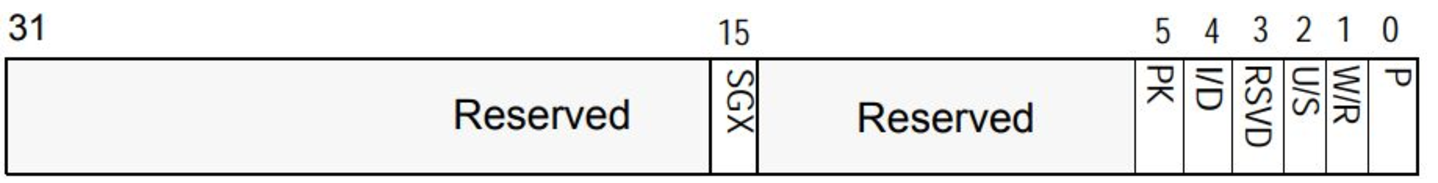
\includegraphics[width=0.47\textwidth]{figures/pagefaulterrorcode2}
  \centering
  \caption{Page Fault Error Code.~\cite{intelinterrupt} \textbf{P}: \textbf{0} The fault was caused by a non-present page; \textbf{1} the fault was caused by a page-level protection violation. \textbf{W/R}: \textbf{0} The access causing the fault was a read; \textbf{1} the fault causing the fault was a write. \textbf{U/S}: \textbf{0} A supervisor-mode access caused the fault; \textbf{1} A user-mode access caused the fault. \textbf{Notice}, there is no exact error code regarding SMAP. In the context of an SMAP exception, the U/S bit is zero, which indicates kernel-mode access. We still need to combine this information with the faulting address and CS segment register to confirm the cause.}
  \label{fig:pagefaulterrorcode}
\end{figure}



We filter out the mitigation-irrelevant exceptions first because they may be nested exceptions caused by our operations, such as page table walking. For example, P:0 in the error code indicates a page absence, and we must pass it to the original page fault handler without any modification. The error code may have multiple bits combined, but we have not observed a SMAP exception on an invalid page so far. The U/S bit and CPL field in the CS segment register reveal whether the kernel caused the exception. Additionally, we keep track of the protected and relevant pages, which helps solve the subsequent conflicts. ~\autoref{algo:pagefaulthandler} shows the basic algorithm to handle the exception.

\begin{algorithm}[ht]
\begin{algorithmic}[1]
\small
\Procedure{PageFaultHandler}{}

\State $address\gets cr2$ 
\State $pte\gets \Call{\textbf{GetPte}}{address}$
\State $teb\gets fs:0x18$

\If{SmapViolation}
	\State $pages[]\gets \Call{\textbf{AddPage}}{$address, pte, cr3, teb$}$
    	\State \Call{\textbf{SetPageKernel}}{pte}
    	\State \Call{\textbf{FlashTlb}}{address}
    	\State \Return{Re-execute}
\ElsIf{UserAccessProtectedPage}
	\If{error.WRITE}
    		\Repeat 
		\State \Call{\textbf{Sleep}}{}
        		\If{\Call{\textbf{CheckPtePermits}}{pte}}
        			\State \Return{Re-execute}
        		\EndIf
        	\Until{$count < 10$}
        	\State \Return{TerminateThread}
	\Else
    		\State \Call{\textbf{SetPgeUserReadonly}}{pte}
    		\State \Call{\textbf{FlashTlb}}{address}
        	\State \Return{Re-execute}
	\EndIf

%%\ElsIf{$user\_write\_readonlypage$}
%%	\If{\Call{HAS\_RECORD}{pte}}
%%    \EndIf

\EndIf
\State \Return{OriginalHandler}
   
\EndProcedure
\end{algorithmic}
\normalsize
\caption{Page Fault Handler}
\label{algo:pagefaulthandler}
\end{algorithm}




\textbf{\textit{Enabling Interrupt in the Page Fault Handler.}} The processor calls the page fault exception as an interrupt gate. Hence when entering the page fault handler, the processor clears EFLAGS: IF bit automatically. It prevents subsequent interruptions from interfering with the handler's execution. Therefore, we first store a copy of the CR2 register.  Then set the IF flag before we walk through the page table because it may contain swapped-out pages, and we need the system brings them back from the disk.


\textbf{\textit{Hypervisor.}} Our light-weight hypervisor set the current system into a guest virtual machine. Unlike a bare-metal hypervisor, it does not emulate hardware devices. All the cores on the physical processor enter the VMX mode, and each core has its VMCS that represents a virtual core in the guest.  

The virtual machine exits to the hypervisor when operating on control registers. To monitor the process context switch, we focus on CR3. When the next process to run is our target, the hypervisor set CR4.SMAP bit in the Guest-state area of VMCS. After re-entering the virtual machine, the SMAP is active on this core. Similarly, the hypervisor disables SMAP if the target process is switched out.


\textbf{\textit{Updating PTE.}} 
Modifications on the page tables need to synchronize with other system components. Typically, the memory management module should hold a global spinlock. However, as a third-party kernel module, we do not have such conditions. In a typical kernel-level TOCTOU attacking scenario, the attacker races with the kernel at full speed. Therefore, our operations should be atomic to avoid conflicts with the kernel. ~\autoref{fig:ptestruct} shows the PTE data structure defined in C code. \texttt{\textcircled{1}} changes the Owner a.k.a U/S bit to zero, which sets this page to kernel-mode. \texttt{\textcircled{2}} is the assembly code generated by a compiler. The one-line C statement becomes three assembly instructions. The problem is that, during the three instructions, the thread may be interrupted or conflicts with other threads that write the same page. It occurs multiple times due to the race conditions when we test exploits against \name, making the mitigation ineffective. To solve this, we use the locked atomic instruction~\cite{intelmanualchapter8}, as shown at \texttt{\textcircled{3}}. 

\begin{figure}[th]
  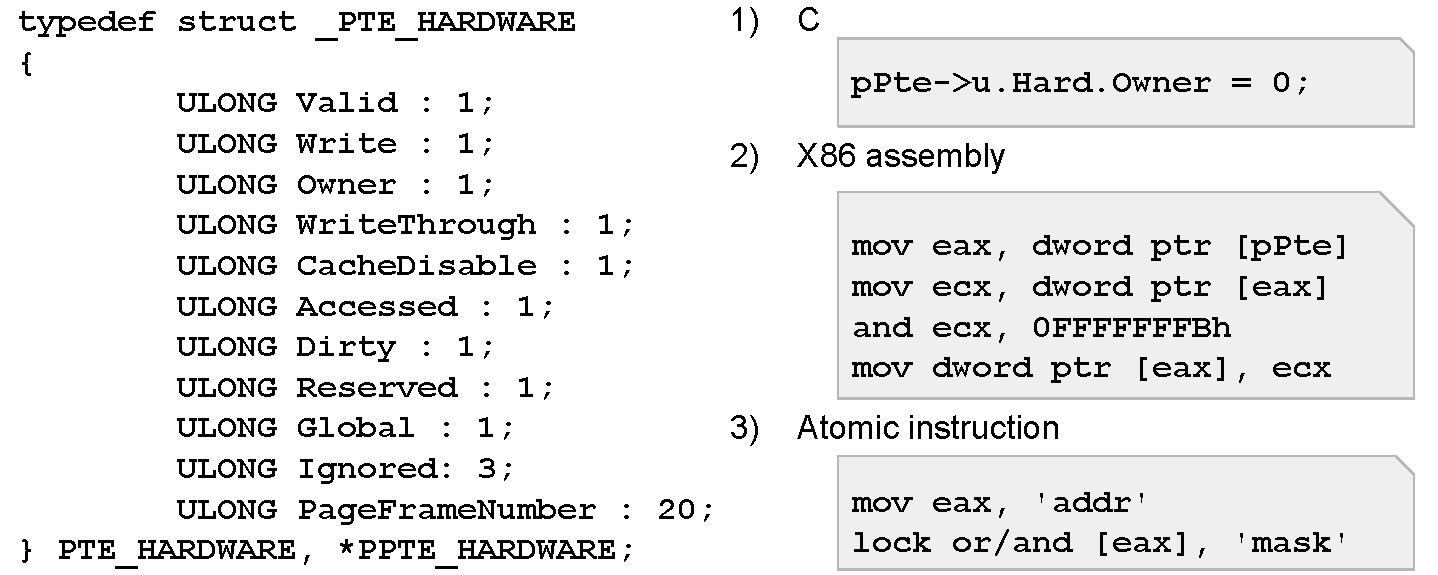
\includegraphics[width=0.47\textwidth]{figures/ptestructcode}
  \centering
  \caption{Left: PTE structure defined in C. Right: C code for changing one bit in the PTE structure, the corresponding assembly code generated by Microsoft C/C++ compiler, and the atomic instructions that serve the same purpose.}
  \label{fig:ptestruct}
\end{figure}


\textbf{\textit{TLB Flushing.}} When we applied our mitigation on real hardware instead of a virtual machine, our mitigation becomes ineffective because we did not flush the TLB.  TLB is a memory cache that stores the recent translation of virtual memory to physical memory. It accelerates the process of accessing virtual memory. Different than data cache, TLB is not entirely transparent to the operating system. When the operating system updates a page table, the corresponding TLB entries need to be invalidated to get new ones.

Instruction \texttt{INVLPG} invalidates a TLB entry, but it only affects the current processor. On a multi-processor system, each core has its TLB. Therefore we need to flush it on every core. For this purpose, we need to issue inter-processor interruption (IPI) to each core through local APIC. The multi-processor system uses IPI messages to distribute interrupts among the processors in the system or execute system-wide functions such as booting up processors or distributing work among a group of processors.

Eventually, we find a Windows kernel internal function, \texttt{KeFlushSingleTb()}. It sends IPI to all processors to invalid a TLB entry.  It calls the hardware abstraction layer (HAL) to send the IPI, so the kernel does not need to care about the actual hardware differences. With this, our mitigation works on the real hardware machine.


\textbf{\textit{Intercepting System Calls.}} As mentioned in~\autoref{sec:ktoctou-design}, to solve read conflicts, \name changes the protected page back to user-mode with a read-only permit. However, since it is no longer a kernel page, the attack can change its permits by calling Win32 APIs. Therefore, we need to intercept system calls  such as \texttt{NtProtectVirtualMemory()} to prevent it. Nevertheless, there may be other ways to go around the system call protection, and we should improve it accordingly. It becomes another arms race between the attacker and the defender, which is out of this paper's scope.



\textbf{\textit{Terminating a Thread.}} When solving the write conflicts, the page fault handler suspends the thread and check the protected page's status periodically. We set a time threshold to avoid deadlock. Therefore, after a few tries, we need to terminate the thread. 

Terminating a thread is not a trivial task. Here we use a trick to let the kernel handle it. We clear the P(present) bit in the PTE and the error code in the kernel stack. Thus, it looks like a thread accesses invalid memory. Then we pass it to the kernel.



\textbf{\textit{Special Cases.}} Windows is a complex operating system. There are always cases that we can not comprehend and need to handle specially. For example, \texttt{USER\_SHARED\_DATA} is a shared page between the kernel and user. Windows maps it at both 0x7FFE0000 and 0xFFDF0000. The kernel frequently reads it because it contains settings such as system time. It is a read-only page, and we treat it differently to improve performance. 
